Una significativa parte del impacto de las computadoras en los distintos aspectos de las
ciencias e incluso de la vida diaria se debe al crecimiento de su
poder de c\'omputo desde la aparici\'on de los primeros microprocesadores hasta el
d\'ia de hoy.

Entre 1986 y 2002, la performance de los procesadores crec\'io en promedio, un 50%
por a\~no~\cite{Pacheco}, en parte gracias a la denominada \textit{Ley de Moore}, que
establec\'ia que la densidad de transistores por circuito integrado se duplicaba
cada 18 meses~\cite{HennessyPatterson}. Esto puede verse en la figura~\ref{processor_performance},
que compara los resultados de los \textit{benchmarks} SPEC de procesadores en distintos
momentos de la historia con respecto al procesador VAX-11/780.

Este crecimiento consistente permiti\'o durante mucho tiempo a los desarrolladores
de aplicaciones escribir programas de manera serial, sabiendo que al poco tiempo los procesadores
mejorar\'ian, y con ellos los tiempos de ejecuci\'on de sus c\'odigos de aplicaci\''on (fen\'omeno denominado
\textit{hardware free lunch}).

\begin{figure}[htbp]
   \centering
   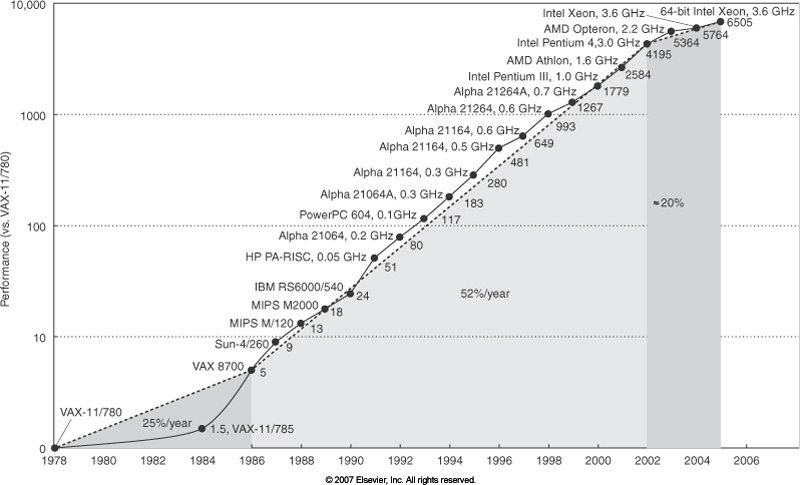
\includegraphics[width=\textwidth]{images/processor-performance.jpg}
   \caption{Performance de procesador en los \textit{benchmarks} SPEC on respecto a VAX-11/780. Tomado de~\cite{HennessyPatterson}}
   \label{processor_performance}
\end{figure}

Sin embargo, a medida que los transistores han disminuido su tama\~no, han incrementado
su disipaci\'on t\'ermica, limitando entonces la cantidad que se puede ubicar de los mismos
en un circuito sin producir que el mismo se comporte de manera err\'atica producto
de la elevada temperatura de operaci\'on. El impacto de esto puede verse en que,
desde 2002, la performance de los monoprocesadores ha visto su crecimiento disminuir
a un 20\%, y consecuentemente se ha modificado el enfoque de dise\~no de procesadores, empezando
a hacerse m\'as y m\'as com\'un el uso de multiprocesadores (multiples procesadores
por chip) para mantener las mejoras de rendimiento.

Esta tendencia puede verse no solo en la continuaci\'on de l\'ineas establecidas
de procesadores (por ejemplo las lineas Intel i3, i5 e i7 de procesadores para computadoras
personales), sino en nuevas arquitecturas que apuntan a computo de alta performance: el incremento
del uso de placas gr\'aficas (GPU) para problemas de computo intensivo, y en desarrollos
nuevos como la arquitectura MIC (\textit{Many Integrated Core Architecture}) de
Intel para coprocesadores num\'ericos.

El impacto de este enfoque hacia multiples hilos de ejecuci\'on en paralelo en el
desarrollo de aplicaciones es significativo. En simulaciones para las \'areas de biolog\'ia,
medicina, qu\'imica o metereolog\'ia es de invaluable utilidad minimizar los tiempos
de ejecuci\'on, para permitir mejores implementaciones de los modelos utilizados,
permitiendo realizar predicciones de mayor calidad. Aprovechar las nuevas
arquitecturas multiprocesador requiere modificaciones en el c\'odigo no triviales,
a diferencia del crecimiento en velocidad de \textit{clock} que no requer\'ia modificaciones
en el dise\~no del programa. Los intentos de escribir programas que conviertan
programas seriales (dise\~nados para un solo procesador) a paralelos, en lenguajes
de prop\'osito general como C, C++ o Fortran, han sido relativamente infructosos.

El resultado es que es necesario trabajo a nivel de escritura del \textit{software}
para utilizar multiples procesadores. La aparici\'on de nuevas herramientas ayudan
al programador en esta tarea. Un ejemplo de esto es Nvidia CUDA (\textit{Compute
Unified Device Architecture}), que provee un lenguaje de programaci\'on unificado
para el desarrollo de aplicaciones que exploten la arquitectura de unidades GPGPU
(\textit{General Purpose Graphical Processing Units}). Otros ejemplos los podemos
ver en APIs y librer\'ias unificadas de desarrollo como OpenMP o MPI
(\textit{Message Passing Interface}), trabajando conjuntamente con compiladores
optimizantes como Intel ICC y PGI Fortran.

Estas herramientas, sin embargo, no son \textit{silver bullets}. Todavia la divisi\'on
del trabajo es inherente al problema a resolver, en base a las dependencias de las tareas
a realizar para la soluci\'on del mismo. Realizar esta division es una labor que, hasta
el dia de hoy, se relega en el programador especializado.

En este trabajo buscaremos comparar distintas arquitecturas de hardware y como
las caracter\'isticas espec\'ificas de la simulaci\'on qu\'imica a realizar permiten
o impiden paralelizaci\'on de trabajo empleando los distintos recursos que cada
arquitectura provee.
